\label{Chapter2}

\section{Μέρος δεύτερο: διαχείριση θορύβου και επιλογή φίλτρων}

Σε αυτό το μέρος της εργασίας, προκείτε να γίνει υποβάθμιση της εικόνας προσθέντονας θορύβο στην αρχική εικόνα και στην συνέχεια να γίνει η επιλογή των καταλλήλων φίλτρων για να επανέλθει στην αρχική της κατάσταση. 
Θόρυβο στην επιστήμη των Σημάτων ονομάζετε τα στοχαστικά σήματα τα οποία έχουν τυχαίες τιμές.
Στην επεξεργασία εικόνας, το σήμα αντιστοιχείτε με το pixel στην οθόνη και ο θορυβός με τις φυσικές καταστάσεις που γίνετε τριγύρω από την φωτογραφία.
Για παράδειγμα, εστώ ότι ένας φωτογράφος τραβάει φωτογραφία ένα ποτάμι. Το πόταμι δεν θα είναι πότε σταθερό.
Θα πρέπει να μπορεί να βρίσκετε σε θέση να αφαιρέσει τον θόρυβο στην φωτογραφία του με την χρήση των καταλλήλων φίλτρων.
Για την εργασία, θα πρέπει να βρεθεί ένας τρόπος ώστε να υποβαθμιστεί η original εικόνα, με σκοπό να επαναφερθεί στην αρχική της κατάσταση.

\subsection{Υποβάθμιση εικόνας με την χρήση θορύβου}

Για να γίνει η υποβάθμιση της εικόνας, θα πρέπει να προσθεθεί ο θόρυβος.

\begin{problem}
	Ποιοι είναι γνωστοί και ευκολοί αλγόριθμοι που μπορούν να υλοποιήθουν ευκόλα για να προσθεθεί ο θόρυβος;
\end{problem}

Οι δύο εύκολοι αλγόριθμοι που μπορούν να χρησιμοποιήθουν είναι ο \textbf{salt and pepper} και ο \textbf{poisson}

\subsubsection{Υλοποίηση του αλγορίθμου salt and pepper}

Ο αλγόριθμος salt and pepper είναι ένας αλγόριθμος ο οποίος δουλεύει πολύ καλά σε ασπρόμαυρες φωτογραφιές.
Όπως φαίνεται και από το όνομα, το salt (δηλάδη το αλάτι, το ασπρό) βρίσκει όλα τα άσπρα σημεία του pepper (πιπέρι, δηλαδή μαύρο) και το pepper το αντίθετο. \par
Ο αλγόριθμος μπορεί να υλοποίηθει με την χρήση του NumPy και του random. Αυτό που κάνει ο αλγόριθμος με λίγα λογία είναι να φτιάχνει ένα αντίγραφο του εικόνας.
Στην συνέχεια, παίρνει έναν τυχαίο αριθμό, τον οποίο τον ελέγχει με ένα όρισμα. Μαθηματικά:

\begin{equation}
	new\_image[i][j] = \Bigg\{
		\begin{tabular}{ccc}
			 0 εάν $ random\_number < probability $ \\
			255 εάν $ random\_number > (1 - probability) $ \\
			αλλίως image[i][j]
		\end{tabular}
\end{equation}

Όπου:

\begin{itemize}
	\item $ noise\_image $ είναι το αντίγραφο της εικόνας
	\item $ probability $ είναι το ορισμά που δέχετε
	\item $ image $ είναι η εικόνα η ίδια
\end{itemize}

Η υλοποίηση στην Python:

\begin{lstlisting}[language=Python, caption=Salt And Pepper]
def salt_and_pepper(image, probability):
    noise_image = np.zeros(image.shape, np.uint8)

    for row in range(image.shape[0]):
        for col in range(image.shape[1]):
            rand = random()
            if rand < probability:
                noise_image[row][col] = 0
            elif rand > (1 - probability):
                noise_image[row][col] = 255
            else:
                noise_image[row][col] = image[row][col]

    return noise_image
\end{lstlisting}

\subsubsection{Υλοποίηση του αλγορίθμου poisson}

\begin{problem}
	``Αν ένα φαινόμενο επαναλαμβάνεται τυχαία στον χρόνο (ή χώρο) με μέσο αριθμό επαναλήψεων λ σε ένα χρονικό (χωρικό) διάστημα, η συνάρτηση πιθανότητας της τυχαίας μεταβλητής $ X $, 
		η οποία μπορεί να είναι ο αριθμός επαναήψεων στο διαστήμα αυτό.

	\begin{equation}
		f_x(x) = e^-l * \frac{\lambda^x}{x!}, x = 0, 1, ...
	\end{equation}
	Στην περίπτωση αυτή, λέμε ότι η $ X $ ακολουθεί \textbf{κατανομή Poisson} με παράμετρο $ \lambda $ και γράφουμε''

	\begin{equation}
		X ~ P_o(\lambda)
	\end{equation}

	(Ν. Μυλωνάς, Β. Παπαδόπουλος)
\end{problem}

Στην επεξεργασία εικόνας, μπορεί να προσθεθεί θόρυβος από την κατανομή του Poisson. To NumPy το έχει ήδη εφαρμοσμένο.

\begin{lstlisting}[language=Python, caption=Poisson]
def poisson(image):
    noise_image = np.random.poisson(image).astype(np.uint8)
    return image + noise_image
\end{lstlisting}

\subsection{Επαναφόρα της εικόνας μέσω φίλτρων}

\begin{problem}
	``Ο όρος φίλτρο έχει προέλθει από την επεξεργασία στο πεδίο της συχνότητας όπου αναφέρεται στην αποδοχή ή την απόρριψη συγκεκριμένων συχνότητων μιας εικόνας.''

	(R. C. Gonzalez, R. E. Woods)
\end{problem}

Για το συγκεκριμένο παράδειγμα, θα πρέπει να αφαιρεθούν με την χρήση τρίων φίλτρων. Τα τρία φίλτρα τα οποία χρησιμοποιούνται είναι το \textbf{Γκαουσιανό φίλτρο}, το \textbf{φίλτρο του μέσου όρου} και το \textbf{φίλτρο της ενδιάμεσης τιμής}.

\subsubsection{Γκαουσιανό φίλτρο}

\begin{problem}
	``Αν το πλήθος των κλάσεων είναι πολύ μεγάλο (τείνει στο άπειρο) και το πλάτος κλάσεων είναι πολύ μικρό (τείνει στο μήδεν), τότε τα πολύγωνα συχνοτήτων παίρνουν τη μορφή μίας ομαλής καμπύλης, οι οποίες ονομάζονται \textbf{καμπύλες συχνοτήτων} ή \textbf{καμπύλες σχετικών συχνοτήτων}.
	Σε πολλές περιπτώσεις μεταβλητών η καμπύλη σχετικών συχνοτήτων έχει μία κωδωνοειδή μορφή. Η καμπύλη αυτή ονομάζεται \textbf{κανονική κατανομή}.''

	(Ν. Μυλωνάς, Β. Παπαδόπουλος)
\end{problem}

Το Γκαουσιανό φίλτρο είναι ένα φίλτρο το οποίο χρησιμοποίει την κανονική κατανομή για να επαναφέρει την εικόνα στην αρχική της κατάσταση. Η βιβλιοθήκη cv2 έχει μερικές συναρτήσεις που υλοποίουν το Γκαουσιανό φίλτρο.

\begin{lstlisting}[language=Python, caption=Gauss Sharp]
kernel = np.ones((5, 5), np.float32) / 25
gauss_image = cv2.GaussianBlur(noise_image, (5, 5), 0)

kernel = np.array(
    [   
        [0, -1, 0],
        [-1, 5, -1],
        [0, -1, 0]
    ]
)

sharp_gauss = cv2.filter2D(gauss_image, -1, kernel)
\end{lstlisting}

\subsubsection{Φίλτρο του μέσου όρου}

Υπάρχουν πολλά φίλτρα μέσου όρου, αλλά αυτός ο οποίος θα χρησιμοποιήθει είναι το φίλτρο αριθμητικού μέσου.

\begin{problem}
	``Το φίλτρο αριθμητικού μέσου αποτελεί και το πιο απλό από τα φίλτρα υπολογισμού του μέσου όρου τιμής.'' 
	(R. C. Gonzalez, R. E. Woods) \par
	Έστω $ S_{xy} $ το σύνολο των συντεταγμένων μίας είκονας $ m * n $ διαστάσεων που έχει κέντρο το $ (x, y) $ Τότε:.

	\begin{equation}
		\hat{f}(x, y) = \frac{1}{m * n} * \sum_{(r, c) \in S_{xy}} g(r, c)
	\end{equation}
\end{problem}

\begin{lstlisting}[language=Python, caption=Average Sharp]
kernel = np.array(
    [   
        [0, -1, 0],
        [-1, 5, -1],
        [0, -1, 0]
    ]
)
average_sharp = cv2.filter2D(noise_image, -1, kernel)
\end{lstlisting}

\subsubsection{Φίλτρο της ενδιάμεσης τιμής}

\begin{problem}
	``Το πιο γνωστό φίλτρο στατιστικής διάταξης είναι το φίλτρο ενδιάμεσης τιμής που αντικαθιστά την τιμή ενός εικονοστοιχείου με την τιμή διάμεσου των επιπέδων έντασης που ανήκουν στη γειτονιά αυτού του εικονοστοιχείου.''
	(R. C. Gonzalez, R. E. Woods)

	\begin{equation}
		\hat{f}(x, y) = median\{g(r, c)\}
	\end{equation}
\end{problem}

\begin{lstlisting}[language=Python, caption=Median Blur]
median_blur = cv2.medianBlur(noise_image, 5)
\end{lstlisting}

\subsection{Εφαρμογή αλγορίθμων}

\subsubsection{Εφαρμογή θορύβων}

Οι αλγόριθμοι πρόκειτε να εφαρμοστούν πάνω στο Σχήμα~\ref{fig:collins}. 
Στον πίνακα~\ref{tab:noise} απεικονίζονται οι νέες εικόνες με τον θόρυβο.
Παρατηρείτε ότι και στις δύο περιπτώσεις, η αρχική εικόνα αλλάζει πάρα πολύ, κυρίως στον Poisson.

\begin{figure}[th]
	\centering
	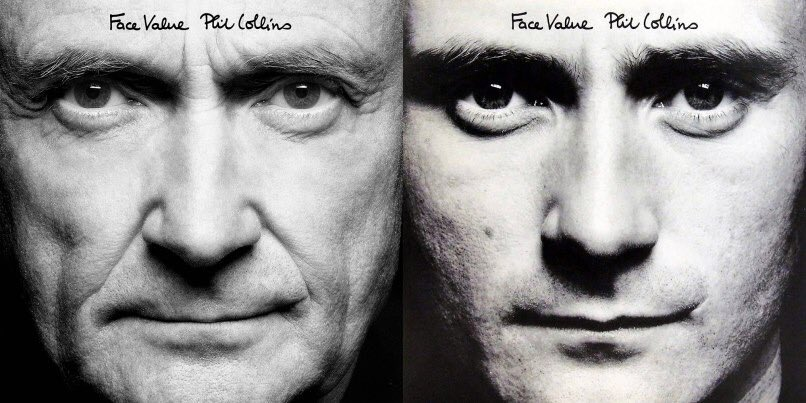
\includegraphics[width=100mm]{Figures/face_value}
	\caption[Phil Collins - Face Value]{Δύο φωτογραφίες του διάσημου frontman και drummer των Genesis, Phil Collins που τραβήχτηκαν σε δύο χρονικές περίοδους για το πρώτο του solo album, Face Value, 1981 και 2015}
	\label{fig:collins}
\end{figure}

\newpage
\begin{table}
	\begin{tabular}{| p{8cm} | p{8cm}|}
		\hline
		\textbf{Salt and Paper} & \textbf{Poisson} \\
		\hline
		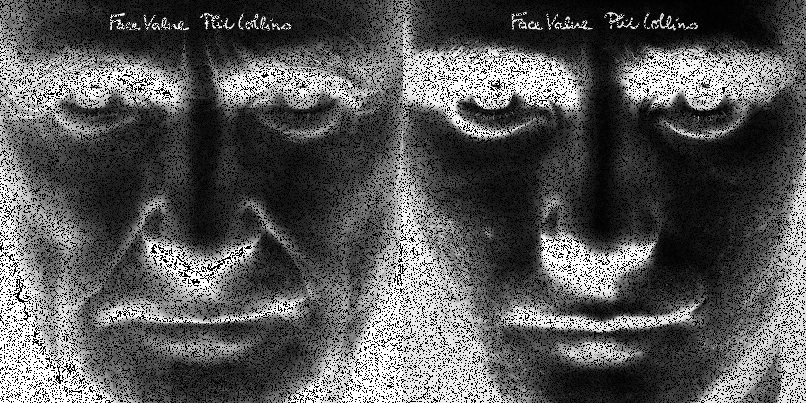
\includegraphics[width=\linewidth]{Figures/sp_noise} &
		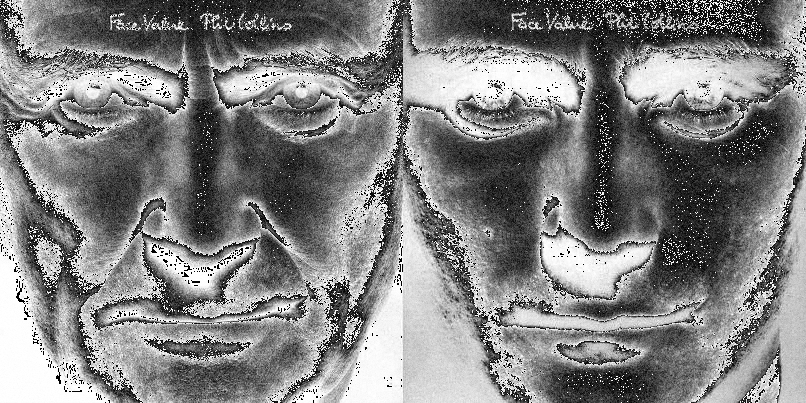
\includegraphics[width=\linewidth]{Figures/poisson_noise} \\
		\hline
	\end{tabular}
	\label{tab:noise}
	\caption{Εφαρμογή των αλγορίθμων του θορύβου στις εικόνες}
\end{table}

\newpage
\subsubsection{Εφαρμογή φίλτρων}

Στον πίνακα~\ref{tab:sp} φαίνονται τα αποτελέσματα από τα φίλτρα στην εικόνα με τον θόρυβο Salt and Pepper, ένω στον πίνακα~\ref{tab:poisson} τα αποτελέσματα από τον Poisson.

\begin{table}
	\begin{tabular}{| p{8cm} | p{8cm}|}
		\hline
		\textbf{Φίλτρο} & \textbf{Εικόνα} \\
		\hline
		Γκαουσιανό φίλτρο &
		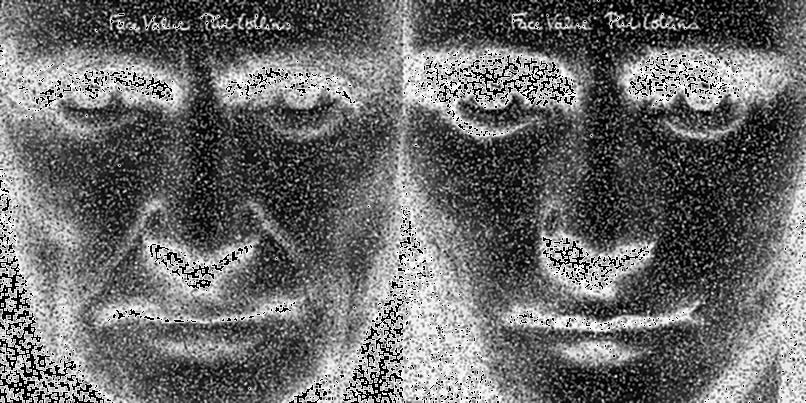
\includegraphics[width=\linewidth]{Figures/sp_gauss_sharp} \\
		\hline
		Φίλτρο μέσου όρου &
		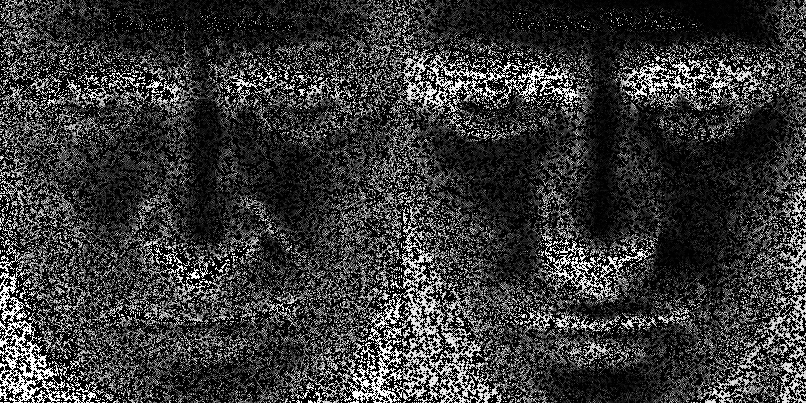
\includegraphics[width=\linewidth]{Figures/sp_average_sharp} \\
		\hline
		Φίλτρο διάμεσης τιμής &
		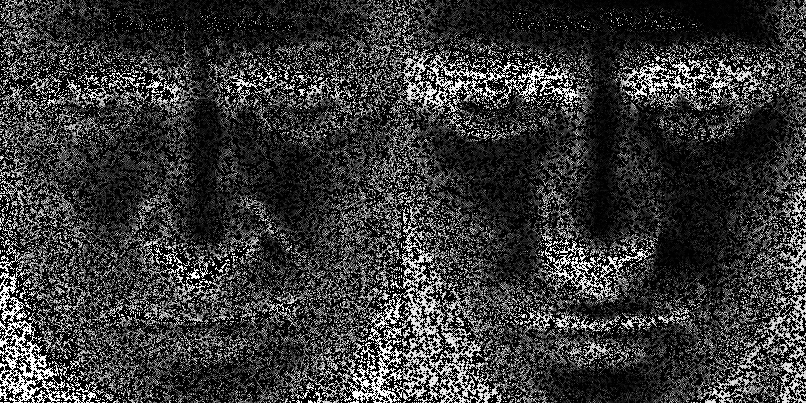
\includegraphics[width=\linewidth]{Figures/sp_median_blur} \\
		\hline
	\end{tabular}
	\label{tab:sp}
	\caption{Εφαρμογή φίλτρων στην είκονα με τον θόρυβο Salt and Paper}
\end{table}

\begin{table}
	\begin{tabular}{| p{8cm} | p{8cm}|}
		\hline
		\textbf{Φίλτρο} & \textbf{Εικόνα} \\
		\hline
		Γκαουσιανό φίλτρο &
		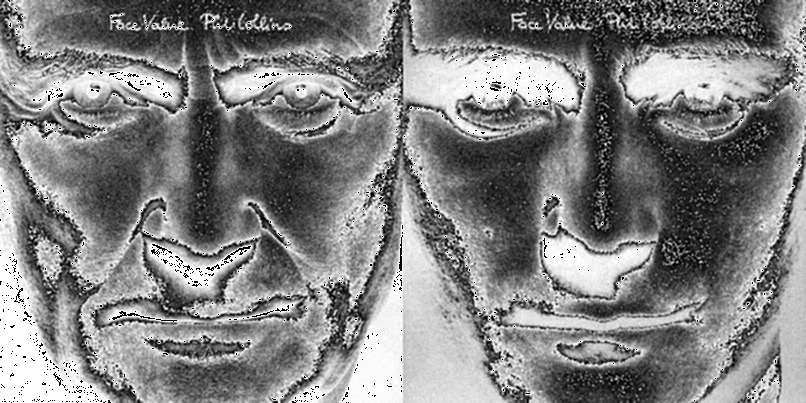
\includegraphics[width=\linewidth]{Figures/poisson_gauss_sharp} \\
		\hline
		Φίλτρο μέσου όρου &
		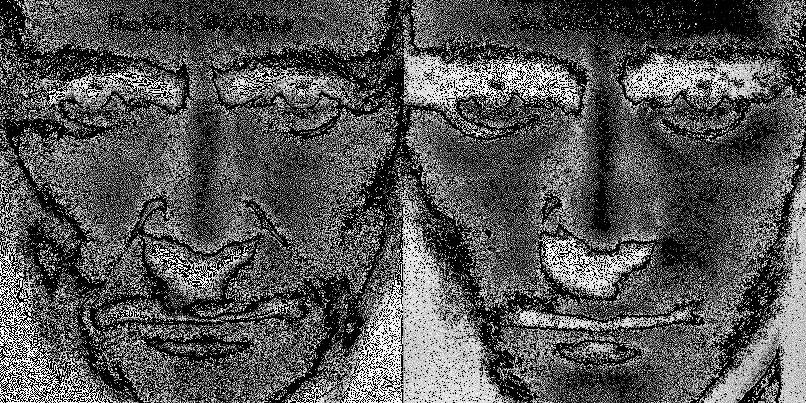
\includegraphics[width=\linewidth]{Figures/poisson_average_sharp} \\
		\hline
		Φίλτρο διάμεσης τιμής &
		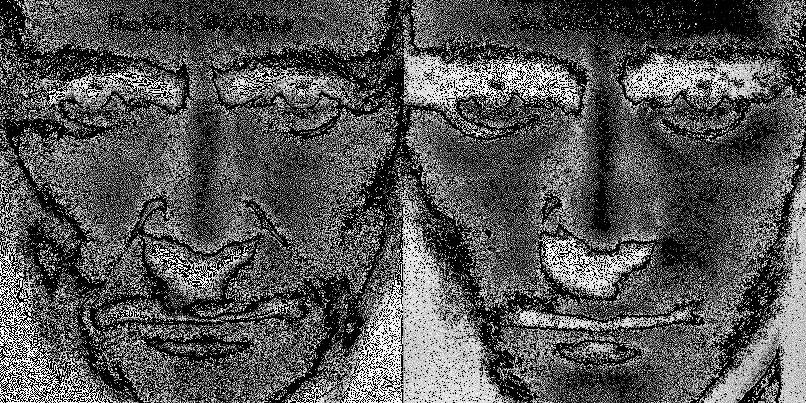
\includegraphics[width=\linewidth]{Figures/poisson_median_blur} \\
		\hline
	\end{tabular}
	\label{tab:poisson}
	\caption{Εφαρμογή φίλτρων στην είκονα με τον θόρυβο Poisson}
\end{table}

\subsection{Σύγκριση με την χρήση αλγοριθμών}

Για το τελεύταιο βήμα, θα χρείαστει να γίνει σύγκριση των είκονων μεταξύ (α) της πρωτότυπης εικόνας με την εξομάλυνση και (β) της εικόνας με τον θόρυβο με την εξομάλυνση.
Οι δύο αλγόριθμοι που θα χρησιμοποιήθουν είναι ο αλγόριθμος \textbf{Structural Similarity Index (SSIM)} και ο \textbf{Mean Square Error}.

\subsubsection{Υλοποίηση του αλγορίθμου SSIM}

Ο αλγόριθμος \textbf{Structural Similarity Index (SSIM)} βρίσκει την διαφορά μεταξύ δύο παρόμοιων εικόνων. Στο skimage.metrics ύπαρχει έτοιμη σύναρτηση όνοματι ssim που το υλοποίει.

\begin{lstlisting}[language=Python, caption=SSIM Algorithm]
def calc_simil(name, original_image, image):
    simil_score, _ = ssim(original_image, image, full=True)
    print(f"{name} SSIM score is: {simil_score}")
\end{lstlisting}

\subsubsection{Υλοποίηση του αλγορίθμου Mean Square Error}

Ο αλγόριθμος \textbf{Mean Square Error} είναι ένας μετρήτης που βρίσκει τον μέσο όρο των λάθων της δύναμης. Ο αλγόριθμος μπορεί να υλοποιηθεί πολύ απλά με το NumPy.

\begin{lstlisting}[language=Python, caption=Mean Squared Error Algorithm]
def calc_mean(name, original_image, image):
    mean_squared_error = np.square(np.subtract(original_image, image)).mean()
    print(f"{name} Mean Squared Error is: {mean_squared_error}")
\end{lstlisting}

\newpage
\subsubsection{Αποτελέσματα}

Τα αποτελέσματα μπορούν να φανούν στους πίνακες~\ref{tab:results_sp_no_noise},~\ref{tab:results_sp_noise},~\ref{tab:results_poisson_no_noise} και~\ref{tab:results_poisson_noise}.

\begin{table}
	\begin{tabular}{| p{2cm} | p{7cm} | p{6.5cm} |}
	\hline
	\textbf{Φίλτρο} & \textbf{Αποτέλεσμα SSIM} & \textbf{Αποτέλεσμα Mean Square Error} \\
	\hline
	Γκαουσιανό φίλτρο & 0.22224864314683754 & 95.79599344863892 \\
	\hline
	Φίλτρο μέσης τιμής & 0.1008267520614758 & 94.49013601462973 \\
	\hline
	Φίλτρο διάμεσης τιμής & 0.7457517695290394 & 40.69571883331589 \\
	\hline
	\end{tabular}
	\label{tab:results_sp_no_noise}
	\caption{Τα αποτελέσματα των συγκρίσεων μετάξυ του πρωτότυπου και της εξομάλυνσης του Salt and Pepper}
\end{table}

\begin{table}
	\begin{tabular}{| p{2cm} | p{7cm} | p{6.5cm} |}
	\hline
	\textbf{Φίλτρο} & \textbf{Αποτέλεσμα SSIM} & \textbf{Αποτέλεσμα Mean Square Error} \\
	\hline
	Γκαουσιανό φίλτρο & 0.5256954158313445 & 94.97967477171832 \\
	\hline
	Φίλτρο μέσης τιμής & 0.8065523248733352 & 73.49161068659988 \\
	\hline
	Φίλτρο διάμεσης τιμής & 0.0813248901272799 & 53.02096866552962 \\
	\hline
	\end{tabular}
	\label{tab:results_sp_noise}
	\caption{Τα αποτελέσματα των συγκρίσεων μετάξυ της εικόνας με τον θόρυβο και της εξομάλυνσης του Salt and Pepper}
\end{table}

\newpage
\begin{table}
	\begin{tabular}{| p{2cm} | p{7cm} | p{6.5cm} |}
	\hline
	\textbf{Φίλτρο} & \textbf{Αποτέλεσμα SSIM} & \textbf{Αποτέλεσμα Mean Square Error} \\
	\hline
	Γκαουσιανό φίλτρο & 0.43015755824644086 & 105.33047737502233 \\
	\hline
	Φίλτρο μέσης τιμής & 0.12037766178876502 & 97.6301775147929 \\
	\hline
	Φίλτρο διάμεσης τιμής & 0.5137574899674178 & 108.9787480989354 \\
	\hline
	\end{tabular}
	\label{tab:results_poisson_no_noise}
	\caption{Τα αποτελέσματα των συγκρίσεων μετάξυ του πρωτότυπου και της εξομάλυνσης του Poisson}
\end{table}

\begin{table}
	\begin{tabular}{| p{2cm} | p{7cm} | p{6.5cm} |}
	\hline
	\textbf{Φίλτρο} & \textbf{Αποτέλεσμα SSIM} & \textbf{Αποτέλεσμα Mean Square Error} \\
	\hline
	Γκαουσιανό φίλτρο & 0.7198557213172727 & 75.2685503882174 \\
	\hline
	Φίλτρο μέσης τιμής & 0.5889702706987753 & 99.21519127634552 \\
	\hline
	Φίλτρο διάμεσης τιμής & 0.42011072522698933 & 78.37677099175538 \\
	\hline
	\end{tabular}
	\label{tab:results_poisson_noise}
	\caption{Τα αποτελέσματα των συγκρίσεων μετάξυ της εικόνας με τον θόρυβο και της εξομάλυνσης του Poisson}
\end{table}

\newpage
\subsection{Συμπεράσματα}

Ο αλγόριθμος Salt and Paper φαίνεται να αλλάζει την εικόνα λιγότερο από την Poisson. 
Στα φίλτρα, το φίλτρο διάμεσης τιμής είναι το καλύτερο φίλτρο, επαναφέρει την εικόνα αρκέτα πιο κοντά από ότι στις υπόλοιπες και αυτό φαίνεται στα αποτελέσματα του SSIM και του Mean Square Error.
